\documentclass[11pt]{article}
\usepackage[a4paper,margin=2.3cm]{geometry}
\usepackage{graphicx,booktabs,array,tabularx,caption,enumitem,microtype}
\usepackage[hidelinks]{hyperref}
\setlist{itemsep=2pt,topsep=4pt}
\captionsetup{font=small,labelfont=bf}
\newcolumntype{Y}{>{\raggedright\arraybackslash}X}
\newcolumntype{C}{>{\centering\arraybackslash}X}
% generated by report/make_numbers.py from the committed result files; do not edit
\newcommand{\boardMem}{16}
\newcommand{\gateHz}{1}
\newcommand{\gateTol}{1.01}
\newcommand{\jerkLimit}{500}
\newcommand{\accLimit}{12}
\newcommand{\budget}{30}
\newcommand{\vOneAttempts}{20}
\newcommand{\nvidiaAttempts}{100}
\newcommand{\vampCommit}{27cb9b6}
\newcommand{\curoboOneCommit}{ebb7170}
\newcommand{\curoboTwoCommit}{ac5f931}
\newcommand{\curoboOneVersion}{v0.7.7-5}
\newcommand{\curoboTwoVersion}{v0.8.0.post1.dev33}
\newcommand{\freezeHash}{6aea6eecf76a}
\newcommand{\reportDate}{2026-10-15}
\newcommand{\agreeN}{16{,}000}
\newcommand{\agreeShare}{100\%}
\newcommand{\vOneRatioMin}{169$\times$}
\newcommand{\vOneRatioMax}{483$\times$}
\newcommand{\vTwoRatioMin}{684$\times$}
\newcommand{\vTwoRatioMax}{3817$\times$}
\newcommand{\pandaVampMs}{1.76\,ms}
\newcommand{\pandaVOneMs}{849\,ms}
\newcommand{\pandaVTwoMs}{6.55\,s}
\newcommand{\pandaVTwoSolved}{59/69}
\newcommand{\pandaVOneOnVTwo}{64/69}
\newcommand{\pandaVOneOnVTwoMs}{869\,ms}
\newcommand{\penMedMin}{0.12}
\newcommand{\penMedMax}{2.30}
\newcommand{\penMax}{5.08}
\newcommand{\urFiveVOneSolved}{367/689}
\newcommand{\feasA}{299}
\newcommand{\feasUnresA}{1}
\newcommand{\feasQA}{300}
\newcommand{\feasMbm}{300}
\newcommand{\feasUnresMbm}{0}
\newcommand{\feasQMbm}{300}
\newcommand{\feasMpi}{299}
\newcommand{\feasUnresMpi}{1}
\newcommand{\feasQMpi}{300}
\newcommand{\feasOrig}{156}
\newcommand{\feasUnresOrig}{144}
\newcommand{\feasQOrig}{300}
\newcommand{\vTwoQueries}{300}
\newcommand{\vTwoSeeds}{10}
\newcommand{\vTwoSubQ}{100}
\newcommand{\vTwoSubSeeds}{3}
\newcommand{\aVampSucc}{93.1\%}
\newcommand{\aVOneSucc}{56.9\%}
\newcommand{\aVTwoSucc}{71.0\%}
\newcommand{\aSubVamp}{95.0\%}
\newcommand{\aSubVOne}{64.7\%}
\newcommand{\aVampCycle}{3.09\,s}
\newcommand{\aVOneCycle}{3.76\,s}
\newcommand{\aBothVamp}{2.67\,s}
\newcommand{\aBothVOne}{2.36\,s}
\newcommand{\aExecAdv}{0.97\,s}
\newcommand{\aReadyAdv}{0.21\,s}
\newcommand{\readyRatioA}{59$\times$}
\newcommand{\readyRatioMbm}{478$\times$}
\newcommand{\readyRatioMpi}{159$\times$}
\newcommand{\readyRatioMin}{59$\times$}
\newcommand{\readyRatioMax}{478$\times$}
\newcommand{\toppraValidMin}{48\%}
\newcommand{\toppraValidMax}{71\%}
\newcommand{\hFiveHolds}{H1, H2, H3 (jerk), H3 (execution time)}
\newcommand{\hFiveFails}{H4}
\newcommand{\vTwoOverVOneMin}{7$\times$}
\newcommand{\vTwoOverVOneMax}{15$\times$}
\newcommand{\ppCells}{30}
\newcommand{\ppPicksPerRun}{600}
\newcommand{\ppPicks}{600}
\newcommand{\ppSeeds}{5}
\newcommand{\ppSegments}{6}
\newcommand{\ppPerCell}{4}
\newcommand{\ppJerkLow}{200}
\newcommand{\ppVampDone}{587/600}
\newcommand{\ppVTwoDone}{585/600}
\newcommand{\ppVOneDone}{0/600}
\newcommand{\ppJDone}{572/600}
\newcommand{\ppVampCycle}{6.08\,s}
\newcommand{\ppVTwoCycle}{18.92\,s}
\newcommand{\ppJCycle}{8.22\,s}
\newcommand{\ppPairTwoN}{576}
\newcommand{\ppPairTwoVamp}{6.07\,s}
\newcommand{\ppPairTwo}{18.88\,s}
\newcommand{\ppPairTwoRatio}{0.32}
\newcommand{\ppPairJN}{566}
\newcommand{\ppPairJVamp}{6.06\,s}
\newcommand{\ppPairJ}{8.22\,s}
\newcommand{\ppPairJRatio}{0.74}
\newcommand{\ppRTwoDone}{573/600}
\newcommand{\ppRTwoCycle}{8.15\,s}
\newcommand{\ppRTwoSlow}{1.27}
\newcommand{\ppMoveLPassOne}{200/2304}
\newcommand{\ttCells}{100}
\newcommand{\ttCandidates}{817}
\newcommand{\ttAccept}{12\%}
\newcommand{\ttViasMin}{3}
\newcommand{\ttViasMax}{6}
\newcommand{\ttViasThree}{52}
\newcommand{\ttViasFour}{24}
\newcommand{\ttViasFive}{13}
\newcommand{\ttViasSix}{11}
\newcommand{\ttSweepMed}{139}
\newcommand{\ttSweepMin}{90}
\newcommand{\ttSweepMax}{269}
\newcommand{\ttRadiusMed}{0.14}
\newcommand{\ttTLenMin}{0.30}
\newcommand{\ttTLenMax}{0.59}
\newcommand{\ttTLenMed}{0.40}
\newcommand{\ttV}{0.25}
\newcommand{\ttA}{1.0}
\newcommand{\ttTA}{0.25}
\newcommand{\ttClearW}{25}
\newcommand{\ttClearC}{14}
\newcommand{\ttClearT}{24}
\newcommand{\ttPathLimit}{5}
\newcommand{\ttEndMm}{1}
\newcommand{\ttEndDeg}{1}
\newcommand{\ttBlendR}{5}
\newcommand{\ttTcpJerk}{10}
\newcommand{\ttInner}{0.35}
\newcommand{\ttOuter}{0.70}
\newcommand{\ttAxisHold}{1}
\newcommand{\ttBinMin}{30}
\newcommand{\ttKnotDt}{40}
\newcommand{\ttLinesW}{483}
\newcommand{\ttLinesWPlane}{15}
\newcommand{\ttLinesWOrient}{468}
\newcommand{\ttLinesWNative}{0}
\newcommand{\ttLinesT}{100}
\newcommand{\ttLinesTPlane}{1}
\newcommand{\ttLinesTOrient}{99}
\newcommand{\ttLinesTNative}{0}
\newcommand{\ttLinesAll}{583}
\newcommand{\ttLinesAllNative}{0}
\newcommand{\ttSeedsVOne}{10}
\newcommand{\ttSeedsVTwo}{3}
\newcommand{\ttCartDevPNinetyFive}{0.04}
\newcommand{\ttCartHalvedW}{76}
\newcommand{\ttCartHalvedC}{15}
\newcommand{\ttCartReadyMin}{0.20}
\newcommand{\ttCartReadyMax}{0.62}
\newcommand{\ttCartCycleW}{7.57}
\newcommand{\ttCuroboSpeedMin}{4.4}
\newcommand{\ttCuroboSpeedMax}{4.9}
\newcommand{\ttCuroboWSpeedMin}{1.5}
\newcommand{\ttCuroboWSpeedMax}{2.0}
\newcommand{\ttCuroboDevMin}{7.6}
\newcommand{\ttCuroboDevMax}{9.3}
\newcommand{\ttCuroboDevSuccMin}{2.3}
\newcommand{\ttCuroboDevSuccMax}{3.6}
\newcommand{\ttCuroboRampMin}{0.18}
\newcommand{\ttCuroboRampMax}{0.23}
\newcommand{\ttLenJShort}{46\%}
\newcommand{\ttLenJLong}{18\%}
\newcommand{\ttPairJN}{34}
\newcommand{\ttPairJ}{1.14}
\newcommand{\ttPairJCart}{2.67}
\newcommand{\ttLenTwoShort}{52\%}
\newcommand{\ttLenTwoLong}{28\%}
\newcommand{\ttPairTwoN}{40}
\newcommand{\ttPairTwo}{1.57}
\newcommand{\ttPairTwoCart}{2.76}
\newcommand{\ttVOneTJerkFail}{898}
\newcommand{\ttVOneTFail}{971}
\newcommand{\ttVOneTDynOnly}{299}
\newcommand{\ttVOneWJerkFail}{1000}
\newcommand{\ttPyReadyW}{41.0}
\newcommand{\ttPyOverW}{79}
\newcommand{\ttPyJerkW}{98}
\newcommand{\ttPyFailW}{99}
\newcommand{\ttPyJerkC}{97}
\newcommand{\ttPyFailC}{97}
\newcommand{\ttPyScaleW}{1.26}
\newcommand{\ttPyScaleC}{1.62}
\newcommand{\ttPyBlendW}{0.95}
\newcommand{\ttPyDevT}{0.21}
\newcommand{\ttPyRampT}{6.8\%}
\newcommand{\ttPySuccT}{84/100}
\newcommand{\ttPyRTwoW}{19/100}
\newcommand{\ttPyRTwoC}{88/100}
\newcommand{\ttPyReadyT}{8.90}
\newcommand{\ttPyExecT}{2.68}
\newcommand{\ttCartSuccAll}{300/300}
\newcommand{\ttTVOne}{29/1000}
\newcommand{\ttWVOne}{0/1000}
\newcommand{\ttTJ}{319/1000}
\newcommand{\ttWJ}{10/1000}
\newcommand{\ttTVTwo}{120/300}
\newcommand{\ttWVTwo}{3/300}
\newcommand{\ttWOneProgram}{1}
\newcommand{\ttStopShare}{100\%}
\newcommand{\moSegs}{480}
\newcommand{\moRecipe}{373/480}
\newcommand{\moPre}{6/480}
\newcommand{\moROne}{0/480}
\newcommand{\moEndRecipe}{475/480}
\newcommand{\moEndPre}{13/480}
\newcommand{\moEndMedRecipe}{0.09}
\newcommand{\moEndMedPre}{2.6}
\newcommand{\moStartOff}{99}
\newcommand{\moStartOnly}{96}
\newcommand{\moGateFail}{6}
\newcommand{\moSolve}{4.55}
\newcommand{\moStartTol}{$10^{-3}$}
\newcommand{\moPicks}{120}
\newcommand{\ikFailFive}{15}
\newcommand{\ikZeroOk}{13}
\newcommand{\ikCtrl}{28}
\newcommand{\ikCtrlColl}{3}
\newcommand{\pyMargin}{5}
\newcommand{\pyKnots}{50}
\newcommand{\ikStarts}{64}
\newcommand{\vOneSeedDump}{168/300}
\newcommand{\marginRule}{most R1 successes, ties to larger margin}
\newcommand{\marginChosen}{5}
\newcommand{\marginQueries}{21}
\newcommand{\marginList}{0\,mm: 7, 5\,mm: 15, 10\,mm: 14, 20\,mm: 5, 50\,mm: 1}

% Every number in this document is a macro from generated/numbers.tex or a table from generated/tab_*.tex,
% both written by report/make_numbers.py from the committed result files. Do not type numbers here.

\title{VAMP, cuRobo and PyRoki on one Jetson Orin NX:\\ planning speed, executable trajectories and industrial motion types}
\author{vamp-bench technical report}
\date{\reportDate}

\begin{document}
\maketitle

\section{Summary}
This report compares motion planners on a single Jetson Orin NX \boardMem\,GB. VAMP is a vectorised sampling-based planner that runs on one CPU core. cuRobo v1 and cuRoboV2 are GPU trajectory optimisers. PyRoki, a JAX trajectory-optimisation library with no global planner, is reported in its own category. All planners check the same collision spheres against the same obstacles and are compared only on this board. The work has three parts.
\begin{itemize}
  \item \textbf{v1} measures planning time on VAMP's standard benchmark and on the scenes of our earlier paper.
  \item \textbf{v2} measures the time to a trajectory that passes a common \gateHz\,kHz executability check, on a held-out set and in pick-place.
  \item \textbf{v2.2} tests motions that cell integrators program: waypoint paths with blends, circular moves (MoveC) and straight lines with a trapezoidal speed profile.
\end{itemize}
Each part was pre-registered before it ran. Changes after registration are logged as amendments.

\paragraph{Takeaways.}
\begin{enumerate}
  \item \textbf{Planning time.} On this board, VAMP on one CPU core plans faster than cuRobo on the whole GPU.
  \begin{itemize}
    \item \textbf{v1:} cuRobo v1's median planning time is \vOneRatioMin\ to \vOneRatioMax\ VAMP's on the same queries, and cuRoboV2's is \vTwoRatioMin\ to \vTwoRatioMax.
    \item \textbf{v2:} counting time-parameterisation, VAMP reaches an executable trajectory \readyRatioMin\ to \readyRatioMax\ sooner than cuRobo v1, in every bin of every set.
  \end{itemize}
  \item \textbf{Cycle time is much closer than planning time}, because execution takes seconds.
  \begin{itemize}
    \item \textbf{Held-out runs both planners solve:} cuRobo v1's cycle is shorter (\aBothVOne\ against \aBothVamp). Its smoother trajectories execute \aExecAdv\ faster, which outweighs VAMP's \aReadyAdv\ planning advantage.
    \item \textbf{Counting failures:} VAMP's median cycle is lower (\aVampCycle\ against \aVOneCycle).
  \end{itemize}
  \item \textbf{The finding of v2.2 is expressibility.} Neither cuRobo version can follow a programmed Cartesian path: it holds a straight line only along an axis of the goal or base frame.
  \begin{itemize}
    \item \textbf{Lines:} none of the \ttLinesAll\ programmed lines runs along such an axis.
    \item \textbf{Other motions:} waypoint paths run as separate lines that stop at every via point. MoveC and a programmed speed profile cannot be expressed.
    \item \textbf{PyRoki:} it expresses all three motion types, and follows the trapezoidal line closely. As returned, its blended and circular trajectories mostly exceed the joint jerk limit.
  \end{itemize}
\end{enumerate}

\section{Setup}
\begin{itemize}
  \item \textbf{Hardware:} one Jetson Orin NX \boardMem\,GB.
  \begin{itemize}
    \item VAMP runs on one Cortex-A78AE core with NEON. cuRobo and PyRoki run on the GPU, with no other GPU work during their runs.
    \item No result here is transferred from other hardware.
  \end{itemize}
  \item \textbf{Planners:}
  \begin{itemize}
    \item VAMP \texttt{\vampCommit} with its library defaults (RRT-Connect, simplification, Halton sampler);
    \item cuRobo v1 \texttt{\curoboOneCommit} (\curoboOneVersion), the version our earlier paper used, with the settings of its own benchmark script;
    \item cuRoboV2 \texttt{\curoboTwoCommit} (\curoboTwoVersion), with NVIDIA's benchmark settings except \texttt{max\_attempts} \vOneAttempts\ instead of \nvidiaAttempts;
    \item PyRoki with its own example settings (Section~\ref{sec:pyroki}).
  \end{itemize}
  \item \textbf{Shared collision model:} all planners use the same sphere model of each robot, the same obstacles and the same joint-space start and goal.
  \begin{itemize}
    \item On \agreeN\ random configurations, VAMP's and cuRobo's collision checkers agree on \agreeShare\ of them.
  \end{itemize}
  \item \textbf{Executability check (v2 onward):} every trajectory, from every planner, is sampled at \gateHz\,kHz and must pass all of the following:
  \begin{itemize}
    \item no collision under the shared model;
    \item joint bounds respected;
    \item peak velocity, acceleration and jerk each at most \gateTol\ times the shared limits.
  \end{itemize}
  The UR5e jerk limit is \jerkLimit\,rad/s\textsuperscript{3}, taken from cuRobo's shipped configuration, since Universal Robots publishes none. Planning plus time-parameterisation (T\textsubscript{ready}) must finish within T $=$ \budget\,s.
  \item \textbf{Two versions of each trajectory:}
  \begin{itemize}
    \item \textbf{R1} is the trajectory as returned.
    \item \textbf{R2} applies a uniform slow-down to a trajectory that failed only on velocity, acceleration or jerk. The factor is the smallest that brings all three peaks within the limits (velocity scales with the factor, acceleration with its square, jerk with its cube). R2 is post-processing and is labelled wherever it appears.
  \end{itemize}
\end{itemize}

\section{v1: planning speed}
\label{sec:v1}
The problem sets are VAMP's MotionBenchMaker problems (Panda, UR5) and the three scenes of our earlier paper (a UR5e on a rail, with and without pillars, and a fixed-base UR5e).
\begin{itemize}
  \item \textbf{Timing:} wall-clock time per query, measured from Python, including the world update.
  \item \textbf{Solved:} the planner reports success.
  \item \textbf{cuRoboV2 subset:} V2 runs a fixed subsample of the MotionBenchMaker problems and one trial per paper problem, because of its run time.
\end{itemize}

\begin{table}[ht]\centering\footnotesize
\caption{Solved queries and wall time per query (median, p95 in parentheses). Rail: the UR5e on a rail of our earlier paper; UR5e: its fixed-base UR5e scene.}\label{tab:v1}
\setlength{\tabcolsep}{4pt}
\begin{tabular}{@{}l rl rl rl@{}}\toprule
 & \multicolumn{2}{c}{VAMP, one CPU core} & \multicolumn{2}{c}{cuRobo v1, GPU} & \multicolumn{2}{c}{cuRoboV2, GPU} \\\midrule
% generated by report/make_numbers.py; do not edit
Panda MBM & 699/699 & 1.76\,ms (3.89) & 638/699 & 849\,ms (2.69\,s) & 59/69 & 6.55\,s (13.9) \\
UR5 MBM & 689/689 & 2.02\,ms (4.80) & 367/689 & 827\,ms (2.18\,s) & 35/64 & 4.52\,s (16.6) \\
Rail, pillars & 1020/1030 & 0.95\,ms (1.35) & 823/1030 & 161\,ms (433) & 100/103 & 1.06\,s (2.28) \\
Rail, no obstacles & 1030/1030 & 0.55\,ms (0.68) & 1030/1030 & 145\,ms (154) & 103/103 & 379\,ms (727) \\
UR5e, pillars & 1030/1030 & 0.97\,ms (1.43) & 985/1030 & 377\,ms (613) & 102/103 & 1.05\,s (2.32) \\
\bottomrule
\end{tabular}
\end{table}

\begin{table}[ht]\centering\footnotesize
\caption{Median wall time relative to VAMP on the same queries.}\label{tab:v1ratio}
\begin{tabularx}{\linewidth}{@{}l CCCCC@{}}\toprule
 & % generated by report/make_numbers.py; do not edit
Panda MBM & UR5 MBM & Rail, pillars & Rail, no obstacles & UR5e, pillars
 \\\midrule
% generated by report/make_numbers.py; do not edit
cuRobo v1 & 483$\times$ & 409$\times$ & 169$\times$ & 261$\times$ & 388$\times$ \\
cuRoboV2 & 3817$\times$ & 2225$\times$ & 1117$\times$ & 684$\times$ & 1079$\times$ \\
\bottomrule
\end{tabularx}
\end{table}

\begin{figure}[ht]\centering
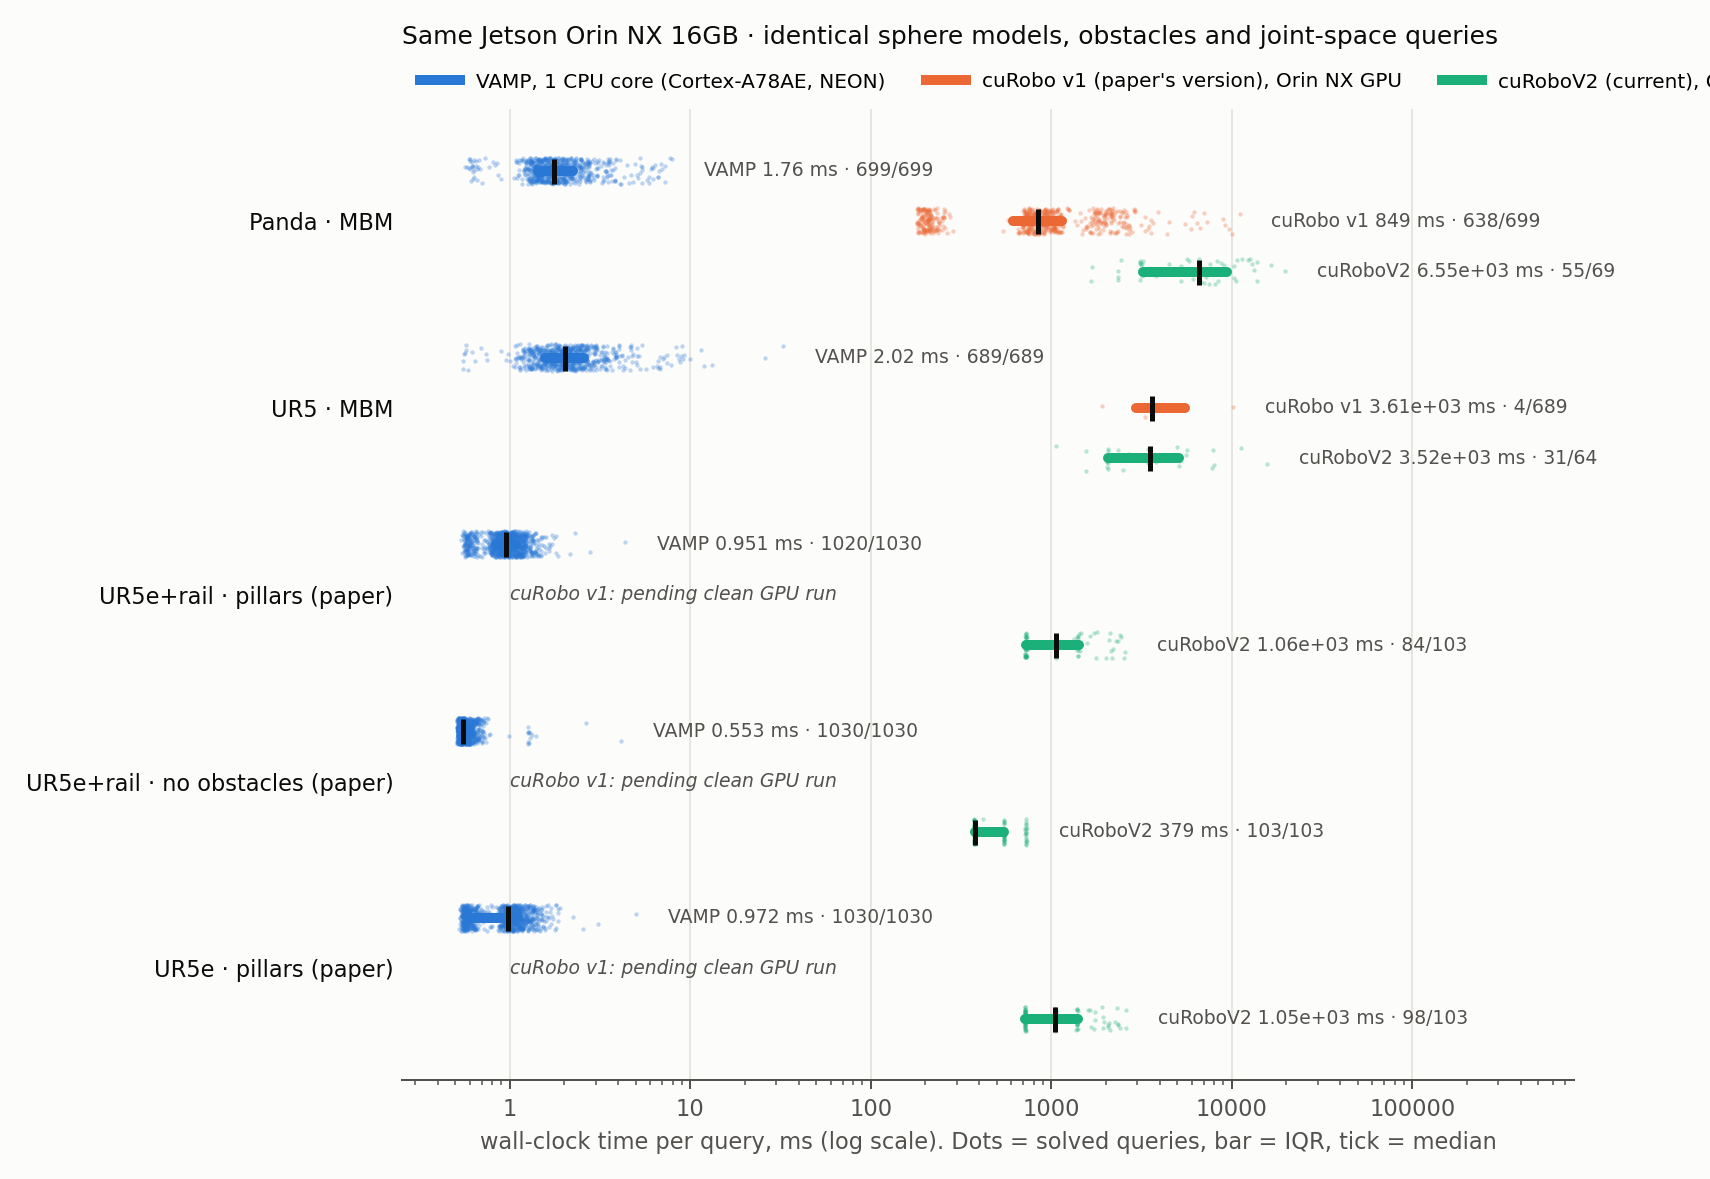
\includegraphics[width=0.92\linewidth]{../results/figure.png}
\caption{Wall-clock time per solved query on each problem set (log scale). Bars show the interquartile range, ticks the median.}\label{fig:v1}
\end{figure}

\paragraph{Panda MotionBenchMaker.}
\begin{itemize}
  \item \textbf{Medians:} VAMP \pandaVampMs, cuRobo v1 \pandaVOneMs, cuRoboV2 \pandaVTwoMs.
  \item \textbf{cuRoboV2's success is a lower bound:} it solves \pandaVTwoSolved\ with \texttt{max\_attempts} \vOneAttempts. NVIDIA's own benchmark uses \nvidiaAttempts.
  \item \textbf{v1 on the same subset:} it solves \pandaVOneOnVTwo\ with a median of \pandaVOneOnVTwoMs.
\end{itemize}
On this board the GPU gives cuRobo no planning-time advantage, and cuRoboV2 is slower than v1.

\paragraph{Notes.}
\begin{itemize}
  \item \textbf{UR5 velocity limit:} VAMP's UR5 model caps every joint at a velocity cuRobo's time-parameterised optimiser cannot work with. Both cuRobo versions therefore receive the real UR5 limit, with identical geometry. cuRobo v1 still solves only \urFiveVOneSolved.
  \item \textbf{Provisional, penetrations between waypoints:} VAMP's straight-line check between consecutive returned waypoints flags a few successes of both cuRobo versions (Table~\ref{tab:flag}).
  \begin{itemize}
    \item \textbf{Size:} median penetration \penMedMin--\penMedMax\,mm per set, at most \penMax\,mm, never at a waypoint.
    \item \textbf{Open question:} whether the continuous cuRobo trajectory itself penetrates is not established.
    \item The solved counts above are not changed.
  \end{itemize}
\end{itemize}

\begin{table}[ht]\centering\footnotesize
\caption{Provisional: successes flagged by VAMP's segment check between returned waypoints.}\label{tab:flag}
\begin{tabular}{@{}lcc@{}}\toprule
 & cuRobo v1 & cuRoboV2 \\\midrule
% generated by report/make_numbers.py; do not edit
Panda MBM & 0 of 638 & 4 of 59 \\
UR5 MBM & 4 of 367 & 6 of 35 \\
Rail, pillars & 44 of 823 & 16 of 100 \\
Rail, no obstacles & 0 of 1030 & 0 of 103 \\
UR5e, pillars & 3 of 985 & 4 of 102 \\
\bottomrule
\end{tabular}
\end{table}

\section{v2: time to an executable trajectory}
\label{sec:v2}
v1 measures time to a path. v2 measures time to a trajectory a controller can execute.
\begin{itemize}
  \item \textbf{What counts:} a planner succeeds only if its output passes the executability check within T $=$ \budget\,s. VAMP's paths are time-parameterised with Ruckig, and the Ruckig time counts.
  \item \textbf{Sets:}
  \begin{itemize}
    \item \textbf{Held-out cells (primary):} \vTwoQueries\ UR5e-on-rail queries generated after a frozen commit. Each query is a pair of collision-free configurations at two stations of a cell, not a tool-down pick.
    \item MotionBenchMaker and M$\pi$Nets Panda queries.
  \end{itemize}
  \item \textbf{Seeds:} \vTwoSeeds\ per query. cuRoboV2 runs a \vTwoSubQ-query subsample with \vTwoSubSeeds\ seeds.
  \item \textbf{Feasibility:} a reference planner certifies \feasA\ of \feasQA\ held-out queries, \feasMbm\ of \feasQMbm\ MotionBenchMaker queries and \feasMpi\ of \feasQMpi\ M$\pi$Nets queries as feasible.
\end{itemize}

\begin{table}[ht]\centering\footnotesize
\caption{Held-out cells (UR5e on a rail). cuRoboV2 on its subsample; on the same runs VAMP succeeds on \aSubVamp\ and cuRobo v1 on \aSubVOne.}\label{tab:v2}
\begin{tabular}{@{}l ccc@{}}\toprule
 & VAMP & cuRobo v1 & cuRoboV2 \\\midrule
% generated by report/make_numbers.py; do not edit
Success (runs) & 93.1\% & 56.9\% & 71.0\% \\
Queries failing on some seed / every seed & 100 / 3 & 160 / 95 & 29 / 29 \\
Median T\textsubscript{ready}, solved runs & 3.54\,ms & 210\,ms & 1.51\,s \\
Median T\textsubscript{exec}, solved runs & 3.03\,s & 2.06\,s & 2.16\,s \\
Median T\textsubscript{cycle} (failures at T) & 3.09\,s & 3.76\,s & 4.06\,s \\
\bottomrule
\end{tabular}
\end{table}

\begin{table}[ht]\centering\footnotesize
\caption{Pre-registered hypotheses H1--H4, per set.}\label{tab:hyp}
\begin{tabular}{@{}p{6.2cm} ccc@{}}\toprule
 & Held-out & MotionBenchMaker & M$\pi$Nets \\\midrule
% generated by report/make_numbers.py; do not edit
H1: VAMP's T\textsubscript{ready} lower in every bin & yes & yes & yes \\
T\textsubscript{ready} ratio, cuRobo v1 / VAMP & 59$\times$ & 478$\times$ & 159$\times$ \\
H2: cycle-time gap smaller (T\textsubscript{cycle} ratio) & yes (1.22) & yes (1.14) & yes (0.99) \\
T\textsubscript{cycle}, runs both solve, VAMP / v1 & 2.67 / 2.36\,s & 2.53 / 3.10\,s & 1.65 / 1.81\,s \\
H3: v1 lower jerk / shorter T\textsubscript{exec} & yes / yes & yes / yes & yes / yes \\
VAMP + TOPP-RA: T\textsubscript{exec}, share valid & 1.79\,s, 48\% & 1.55\,s, 56\% & 1.14\,s, 71\% \\
H4: queries failing on some seed, VAMP / v1 & 100 / 160 & 231 / 55 & 128 / 17 \\
H4: more robust & VAMP & cuRobo v1 & cuRobo v1 \\
\bottomrule
\end{tabular}
\end{table}

\paragraph{Results.}
\begin{itemize}
  \item \textbf{Time to an executable trajectory:} VAMP reaches one \readyRatioA\ (held-out), \readyRatioMbm\ (MotionBenchMaker) and \readyRatioMpi\ (M$\pi$Nets) sooner than cuRobo v1 in median. This holds in every bin of every set (Figure~\ref{fig:bins}).
  \item \textbf{Cycle time:} the gap is far smaller (Table~\ref{tab:hyp}, H2).
  \begin{itemize}
    \item \textbf{Held-out runs both planners solve:} cuRobo v1's cycle is shorter, because its execution is shorter.
    \item \textbf{Counting failures at T:} VAMP's median cycle is lower.
  \end{itemize}
  \item \textbf{Smoothness:} cuRobo v1's trajectories have lower jerk and shorter execution than VAMP with Ruckig, on every set (H3).
  \begin{itemize}
    \item \textbf{VAMP with TOPP-RA:} it executes faster, but only \toppraValidMin\ to \toppraValidMax\ of its trajectories pass the check.
  \end{itemize}
  \item \textbf{Robustness differs by set (H4):} VAMP has fewer queries failing on some seed on the held-out set, and cuRobo v1 has fewer on MotionBenchMaker and M$\pi$Nets.
  \item \textbf{cuRoboV2:} its median T\textsubscript{ready} is \vTwoOverVOneMin\ to \vTwoOverVOneMax\ cuRobo v1's on the same queries and seeds.
  \item \textbf{Appendix set (H5):} on the held-out set with its original, unwrapped goals, \feasOrig\ of \feasQOrig\ queries are certified. The signs of \hFiveHolds\ agree with the primary set; \hFiveFails\ does not.
\end{itemize}

\begin{figure}[ht]\centering
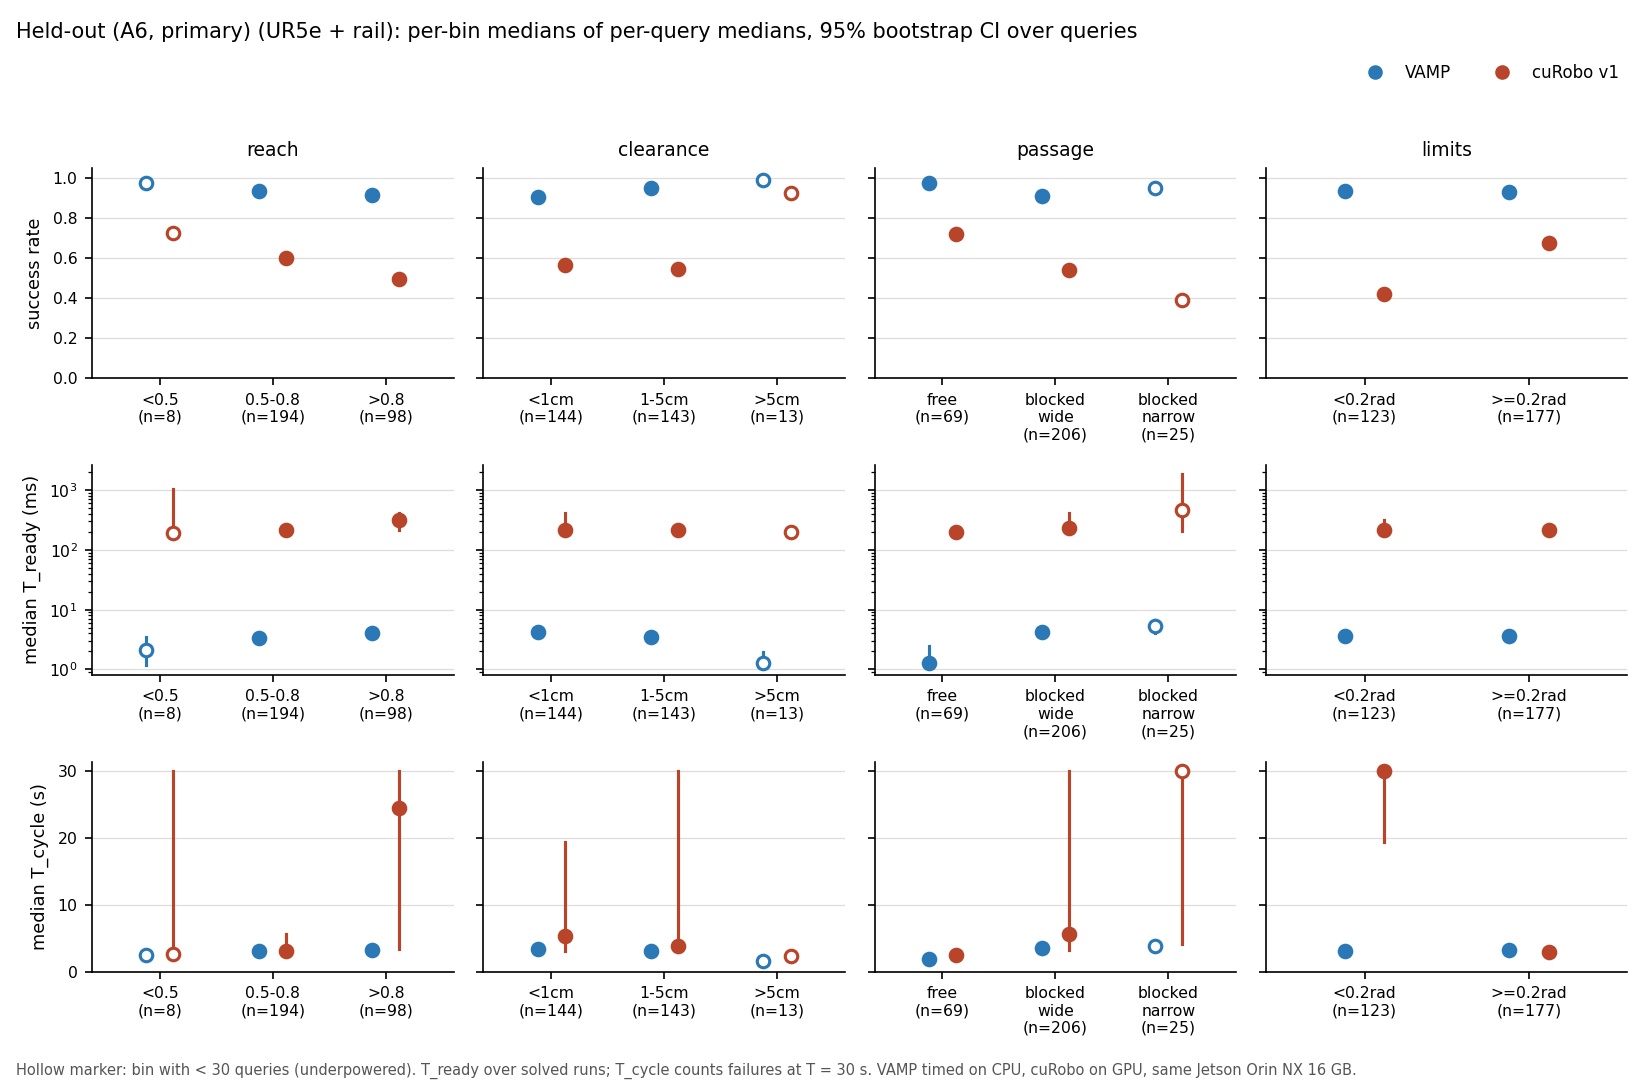
\includegraphics[width=\linewidth]{../results/v2/per_bin_heldout_a6.png}
\caption{Held-out cells: success rate, T\textsubscript{ready} and T\textsubscript{cycle} per bin, with bootstrap confidence intervals over queries. Hollow markers are bins with fewer than \ttBinMin\ queries.}\label{fig:bins}
\end{figure}

\subsection{Pick-place with straight-line approach and retreat}
\begin{itemize}
  \item \textbf{Task:} \ppCells\ cells with \ppPerCell\ picks each, run with \ppSeeds\ seeds, for \ppPicks\ picks per planner.
  \item \textbf{Picks:} each pick has \ppSegments\ segments: free-space moves to the pre-grasp and pre-place poses, and straight-line (MoveL) moves down and up at each.
  \item \textbf{Success:} a pick counts only if every segment passes the check.
\end{itemize}

\begin{table}[ht]\centering\footnotesize
\caption{Pick-place with MoveL (UR5e on a rail).}\label{tab:pp}
\begin{tabular}{@{}p{5.2cm} cccc@{}}\toprule
 & % generated by report/make_numbers.py; do not edit
VAMP & v1 as configured & v1, max\_jerk 200 & cuRoboV2
 \\\midrule
% generated by report/make_numbers.py; do not edit
Picks completed & 587/600 & 0/600 & 572/600 & 585/600 \\
Pick slots failing on some seed & 8/120 & 120/120 & 11/120 & 3/120 \\
Median cycle per completed pick & 6.08\,s & -- & 8.22\,s & 18.92\,s \\
\quad planning & 0.35\,s & -- & 2.76\,s & 13.71\,s \\
\quad execution & 5.72\,s & -- & 5.47\,s & 5.34\,s \\
MoveL TCP deviation, median / p95 (mm) & 0.04 / 0.07 & 0.04 / 0.49 & 0.03 / 0.34 & 0.65 / 0.92 \\
MoveL orientation deviation, p95 & 0.03$^\circ$ & 1.89$^\circ$ & 1.51$^\circ$ & 0.05$^\circ$ \\
\bottomrule
\end{tabular}
\end{table}

\paragraph{Results.}
\begin{itemize}
  \item \textbf{Picks completed:} VAMP \ppVampDone, cuRoboV2 \ppVTwoDone, cuRobo v1 as configured \ppVOneDone.
  \item \textbf{cuRobo v1 as configured:} its MoveL trajectories exceed its own configured jerk limit at the segment ends (Figure~\ref{fig:jerk}). Only \ppMoveLPassOne\ of its MoveL segments pass.
  \begin{itemize}
    \item \textbf{Lower jerk setting:} with \texttt{max\_jerk} lowered to \ppJerkLow, it completes \ppJDone.
    \item \textbf{Uniform slow-down (R2, post hoc):} with a median factor of \ppRTwoSlow\ it completes \ppRTwoDone\ at a median cycle of \ppRTwoCycle.
  \end{itemize}
  \item \textbf{Paired cycle times:}
  \begin{itemize}
    \item \textbf{VAMP and cuRoboV2} (\ppPairTwoN\ picks both complete): \ppPairTwoVamp\ against \ppPairTwo, a median ratio of \ppPairTwoRatio.
    \item \textbf{VAMP and the v1 control} (\ppPairJN\ picks): \ppPairJVamp\ against \ppPairJ, a ratio of \ppPairJRatio.
  \end{itemize}
  Execution times are close, so the differences are planning time.
  \item \textbf{Timing caveat:} VAMP's pick-place planning ran while other jobs loaded the CPU, so its planning times are upper bounds.
\end{itemize}

\begin{figure}[ht]\centering
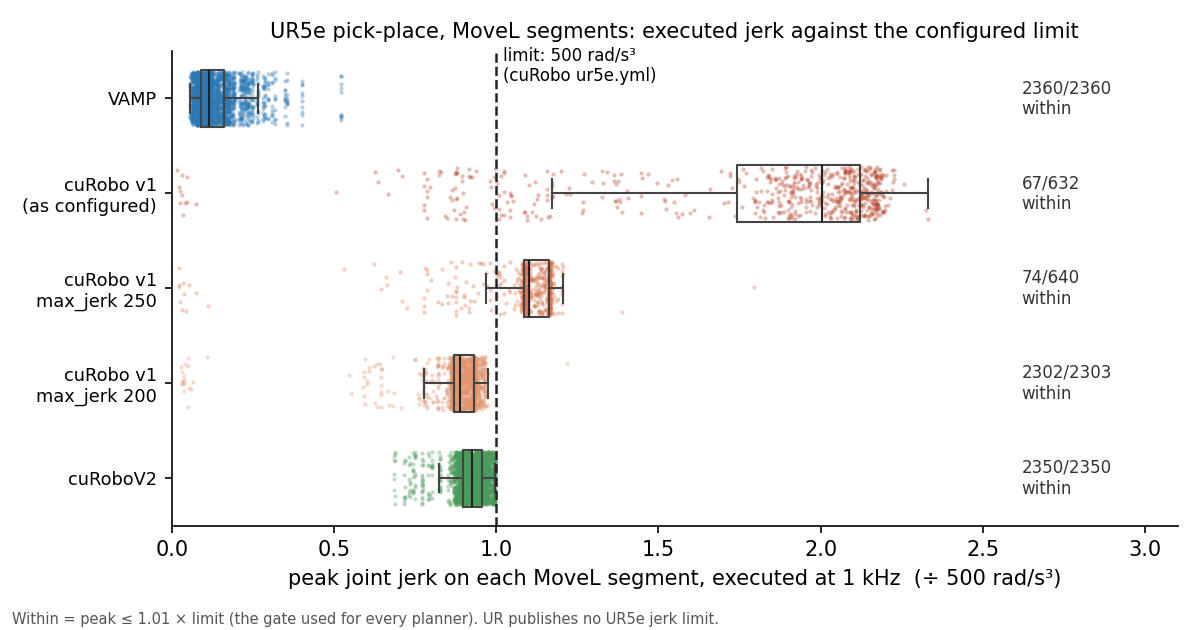
\includegraphics[width=0.85\linewidth]{../results/v2/pickplace_jerk.png}
\caption{Peak joint jerk on each executed MoveL segment, relative to the configured limit.}\label{fig:jerk}
\end{figure}

\section{v2.2: industrial motion types}
\label{sec:v22}
\paragraph{Programs.} \ttCells\ UR5e cells each carry three programmed tool-down motions:
\begin{itemize}
  \item \textbf{W:} a path through \ttViasMin--\ttViasMax\ via points with circular blends (radius up to \ttBlendR\,cm), at a constant \ttV\,m/s through the blends;
  \item \textbf{C:} a horizontal circular arc through start, via and end points (MoveC);
  \item \textbf{T:} a straight line of \ttTLenMin--\ttTLenMax\,m with a trapezoidal TCP speed profile (acceleration \ttTA\,m/s\textsuperscript{2}, cruise \ttV\,m/s).
\end{itemize}
Each time law is jerk-limited along the path (TCP jerk \ttTcpJerk\,m/s\textsuperscript{3}).

\paragraph{Success.} A run must pass all of the following:
\begin{itemize}
  \item the executability check;
  \item planning within T;
  \item an end pose within \ttEndMm\,mm and \ttEndDeg$^\circ$;
  \item a TCP within \ttPathLimit\,mm of the programmed path outside blend zones, with orientation within \ttEndDeg$^\circ$.
\end{itemize}
Speed, blend and profile behaviour are measured but are not part of success, because some planners have no speed input.

\paragraph{Runs.} cuRobo v1 ran with \ttSeedsVOne\ seeds per program, both as configured and with \texttt{max\_jerk} lowered as in pick-place. cuRoboV2 ran with \ttSeedsVTwo\ seeds, and PyRoki once (it is deterministic).

\paragraph{Cartesian pipeline.} This column is our own path IK, spline and time law, with VAMP used only as the collision check. It is a reference for what the programmed motion costs on this robot, not a result about VAMP's planning.

\subsection{Expressibility}
\begin{table}[ht]\centering\footnotesize
\caption{How each planner expresses each motion type. This is the main v2.2 result.}\label{tab:expr}
\begin{tabularx}{\linewidth}{@{}p{2.2cm} YYY@{}}\toprule
Motion & cuRobo v1 and cuRoboV2 & PyRoki & Cartesian pipeline \\\midrule
W, waypoints with blends & Closest native motion: one line per leg, stopping at each via point. Of \ttLinesW\ legs, \ttLinesWNative\ run along a holdable axis, \ttLinesWPlane\ can hold one axis, and \ttLinesWOrient\ hold orientation only. & Per-knot pose costs (our harness) & Our post-processing \\
C, MoveC & Not expressible; not run & Per-knot pose costs & Our post-processing \\
T, trapezoidal line & Line only, by the same rule: of \ttLinesT\ lines, \ttLinesTNative\ along an axis, \ttLinesTPlane\ plane, \ttLinesTOrient\ orientation only. The speed profile is not expressible (no TCP speed or acceleration input). & Per-knot targets at the programmed timing & Our post-processing; profile exact \\
\bottomrule\end{tabularx}
\end{table}

\begin{itemize}
  \item \textbf{How cuRobo holds a line:} both versions hold a straight line by holding axes of the goal frame or the base frame. An axis can be held only when the line's displacement along it is at most \ttAxisHold\,mm.
  \begin{itemize}
    \item A tool-down line in an arbitrary direction usually has no such axis. Only orientation is then held, and the TCP path between the endpoints is unconstrained.
  \end{itemize}
  \item \textbf{cuRoboV2's per-timestep targets:} its interface documents per-timestep tool-pose targets, but its trajectory optimiser rejects a goal of more than one timestep. A probe on development cells, logged before the measured runs, confirmed this.
  \item \textbf{What the cuRobo results measure:} cuRobo runs these programs through its closest native motion. Its results below measure that gap, not its free-space planning.
\end{itemize}

\subsection{Results per motion type}
\begin{table}[ht]\centering\footnotesize
\caption{W, waypoint paths with blends (\ttCells\ programs).}\label{tab:w}
\begin{tabularx}{\linewidth}{@{}p{4.1cm} CCCCC@{}}\toprule
 & % generated by report/make_numbers.py; do not edit
Cartesian pipeline & cuRobo v1 & v1, max\_jerk 200 & cuRoboV2 & PyRoki
 \\\midrule
% generated by report/make_numbers.py; do not edit
Success, as returned (R1) & 100/100 & 0/1000 & 10/1000 & 3/300 & 1/100 \\
Success after slow-down (R2) & 100/100 & 10/1000 & 10/1000 & 3/300 & 19/100 \\
Programs failing on every seed & 0 & 100 & 99 & 99 & 99 \\
Max path deviation, all runs, median / p95 (mm) & 0.03 / 0.04 & 24.35 / 154.26 & 24.36 / 155.74 & 23.42 / 457.93 & 1.82 / 3.78 \\
Cruise speed / programmed, median & 0.50 & 1.98 & 1.69 & 1.54 & 0.99 \\
Via points: median min speed / programmed & 0.50 & 0.00 & 0.00 & 0.00 & 0.95 \\
Via points stopped / held & 0\% / 22\% & 100\% / 0\% & 100\% / 0\% & 100\% / 0\% & 0\% / 73\% \\
Median planning time, all runs & 0.62\,s & 2.63\,s & 2.64\,s & 4.21\,s & 41.00\,s \\
\bottomrule
\end{tabularx}
\end{table}
\begin{table}[ht]\centering\footnotesize
\caption{C, circular arcs (\ttCells\ programs).}\label{tab:c}
\begin{tabularx}{\linewidth}{@{}p{4.1cm} CCCCC@{}}\toprule
 & % generated by report/make_numbers.py; do not edit
Cartesian pipeline & cuRobo v1 & v1, max\_jerk 200 & cuRoboV2 & PyRoki
 \\\midrule
% generated by report/make_numbers.py; do not edit
Success, as returned (R1) & 100/100 & not expressible & not expressible & not expressible & 3/100 \\
Success after slow-down (R2) & 100/100 & -- & -- & -- & 88/100 \\
Programs failing on every seed & 0 & -- & -- & -- & 97 \\
Max path deviation, all runs, median / p95 (mm) & 0.03 / 0.04 & -- & -- & -- & 1.21 / 4.72 \\
Cruise speed / programmed, median & 1.00 & -- & -- & -- & 1.00 \\
Median planning time, all runs & 0.20\,s & -- & -- & -- & 11.72\,s \\
\bottomrule
\end{tabularx}
\end{table}
\begin{table}[ht]\centering\footnotesize
\caption{T, straight lines with a trapezoidal profile (\ttCells\ programs).}\label{tab:t}
\begin{tabularx}{\linewidth}{@{}p{4.1cm} CCCCC@{}}\toprule
 & % generated by report/make_numbers.py; do not edit
Cartesian pipeline & cuRobo v1 & v1, max\_jerk 200 & cuRoboV2 & PyRoki
 \\\midrule
% generated by report/make_numbers.py; do not edit
Success, as returned (R1) & 100/100 & 29/1000 & 319/1000 & 120/300 & 84/100 \\
Success after slow-down (R2) & 100/100 & 328/1000 & 319/1000 & 120/300 & 99/100 \\
Programs failing on every seed & 0 & 91 & 66 & 60 & 16 \\
Max path deviation, all runs, median / p95 (mm) & 0.03 / 0.04 & 9.27 / 39.20 & 9.01 / 39.13 & 7.59 / 28.10 & 0.21 / 1.08 \\
Cruise speed / programmed, median & 1.00 & 4.93 & 4.63 & 4.36 & 1.00 \\
Ramp acceleration error, median & 2\% & 2646\% & 2257\% & 2083\% & 7\% \\
Ramp duration / programmed, median & 1.00 & 0.18 & 0.20 & 0.23 & 1.00 \\
Median T\textsubscript{cycle}, successful runs & 2.90\,s & 1.22\,s & 1.14\,s & 1.57\,s & 11.64\,s \\
Median planning time, all runs & 0.25\,s & 0.61\,s & 0.63\,s & 1.02\,s & 9.02\,s \\
\bottomrule
\end{tabularx}
\end{table}

\begin{figure}[ht]\centering
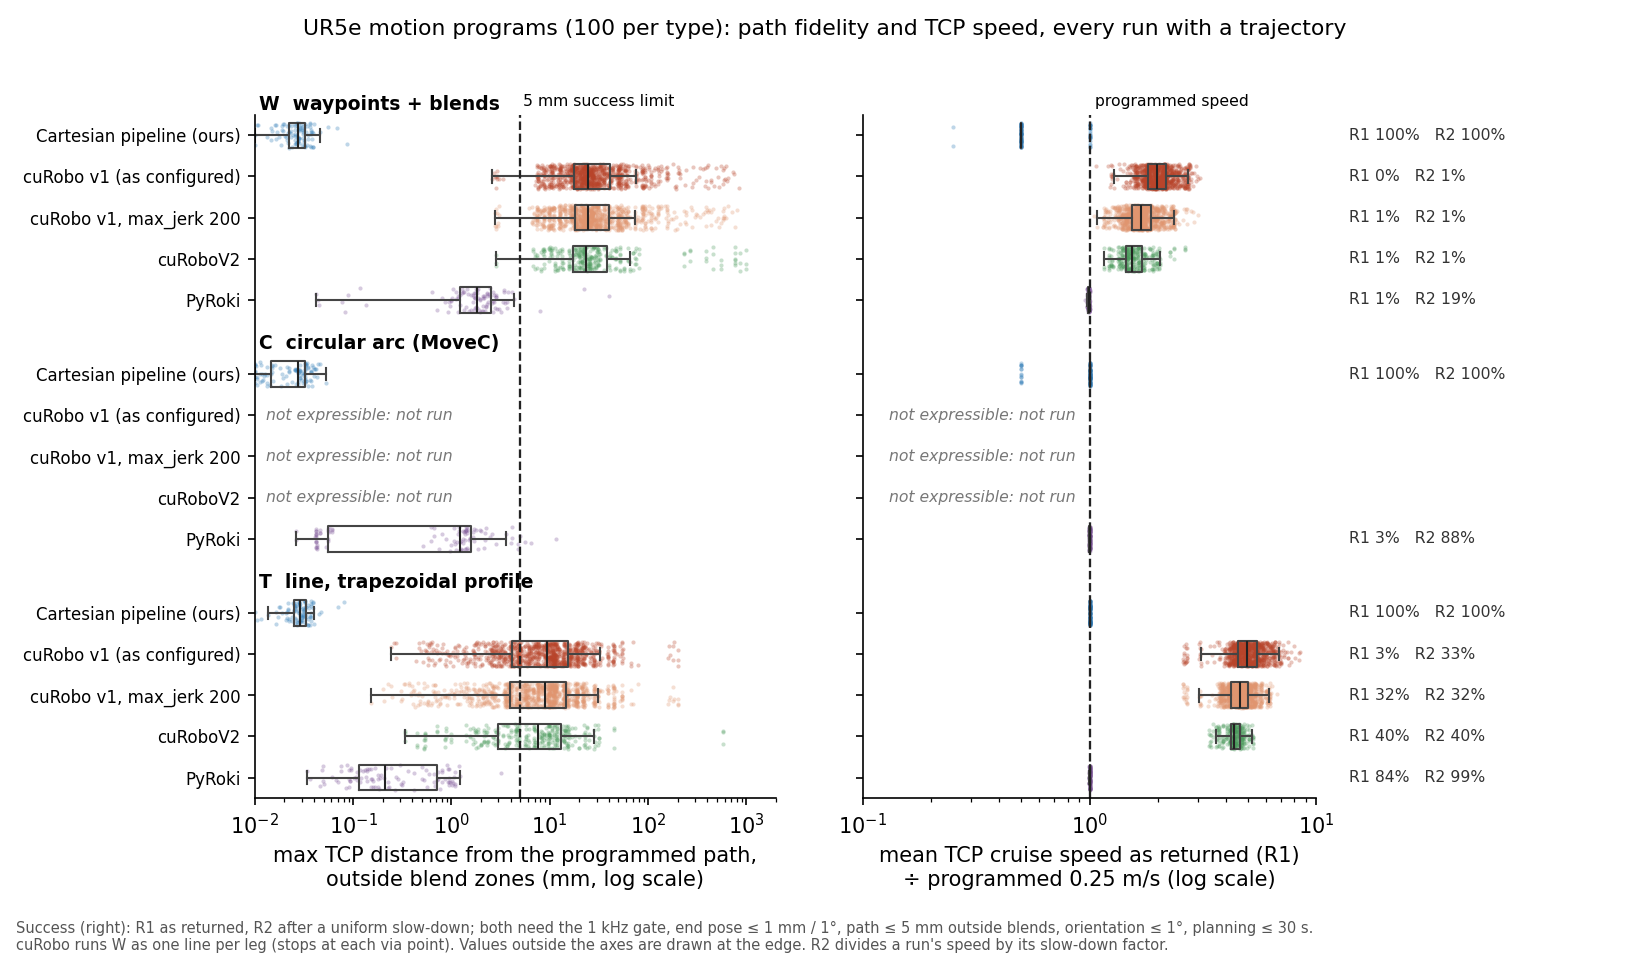
\includegraphics[width=\linewidth]{../results/v2_2/motion_types.png}
\caption{Path deviation outside blend zones (left) and cruise speed relative to the programmed speed (right), for every run with a trajectory.}\label{fig:v22}
\end{figure}

\paragraph{cuRobo.}
\begin{itemize}
  \item \textbf{Waypoint paths:} one program succeeds (\ttWVTwo\ for cuRoboV2, \ttWJ\ for v1 with the lower jerk setting). Its legs all hold orientation only and happen to stay within the path limit. Every cuRobo waypoint path stops at the via points.
  \item \textbf{T lines:} cuRoboV2 succeeds on \ttTVTwo\ runs, v1 with the lower jerk setting on \ttTJ\ and v1 as configured on \ttTVOne.
  \begin{itemize}
    \item \textbf{Path:} over all runs the median maximum deviation is \ttCuroboDevMin--\ttCuroboDevMax\,mm. On successful runs it is \ttCuroboDevSuccMin--\ttCuroboDevSuccMax\,mm, so the pre-registered path-fidelity mark (median at most \ttEndMm\,mm) is not met.
    \item \textbf{Speed:} cuRobo moves the line at its own time-optimal speed, \ttCuroboSpeedMin\ to \ttCuroboSpeedMax\ times the programmed speed in median. Its ramps last \ttCuroboRampMin--\ttCuroboRampMax\ of the programmed duration.
    \item \textbf{Cycle time:} its cycle is shorter than the Cartesian pipeline's on the programs both solve (cuRoboV2 \ttPairTwo\,s against \ttPairTwoCart\,s over \ttPairTwoN\ programs). That cycle is not the cycle of the programmed motion.
    \item \textbf{Line length:} success falls with length. cuRoboV2 succeeds on \ttLenTwoShort\ of runs on lines shorter than the median and \ttLenTwoLong\ on longer ones; for v1 with the lower jerk setting the figures are \ttLenJShort\ and \ttLenJLong.
  \end{itemize}
  \item \textbf{cuRobo v1 as configured:} as in pick-place, its trajectories exceed the jerk limit (\ttVOneTJerkFail\ of \ttVOneTFail\ failed T runs).
\end{itemize}

\paragraph{PyRoki.}
\begin{itemize}
  \item \textbf{T lines:} it succeeds on \ttPySuccT, with a median deviation of \ttPyDevT\,mm and a ramp acceleration error of \ttPyRampT.
  \begin{itemize}
    \item \textbf{Cycle time:} planning dominates (\ttPyReadyT\,s planning, \ttPyExecT\,s execution).
  \end{itemize}
  \item \textbf{W and C, as returned:} the trajectories keep the programmed speed, including through the blends (median via-point speed \ttPyBlendW\ of programmed). But \ttPyJerkW\ of \ttPyFailW\ failed W runs and \ttPyJerkC\ of \ttPyFailC\ failed C runs exceed the jerk limit.
  \item \textbf{W and C after slow-down (R2):} \ttPyRTwoW\ (W) and \ttPyRTwoC\ (C) succeed, at median slow-downs of \ttPyScaleW\ and \ttPyScaleC, so below the programmed speed.
  \item \textbf{Planning time on W:} with knots at most \ttKnotDt\,ms apart, W planning takes a median of \ttPyReadyW\,s, and \ttPyOverW\ programs exceed T.
\end{itemize}

\paragraph{Cartesian pipeline.}
\begin{itemize}
  \item \textbf{Fidelity and planning time:} it completes \ttCartSuccAll\ programs and holds every path to \ttCartDevPNinetyFive\,mm (p95). Planning takes a median of \ttCartReadyMin--\ttCartReadyMax\,s per program type.
  \item \textbf{Speed:} at the programmed speed, the circular blends exceed the joint limits on \ttCartHalvedW\ of \ttCells\ waypoint paths, and so do \ttCartHalvedC\ arcs. By the pre-registered rule it then halves the program speed.
  \item \textbf{Cycle time on W:} its median is \ttCartCycleW\,s, including the halved speed.
\end{itemize}

\section{v2.1: PyRoki as a trajectory optimiser (provisional)}
\label{sec:pyroki}
\noindent\textbf{Status: provisional.} The v2.1 write-up is pending. These numbers come from the stored runs, summarised by a script, and may be revised.

\paragraph{Correction first: MoveL succeeds on \moRecipe\ segments, not \moPre.}
\begin{itemize}
  \item \textbf{The setup:} PyRoki ran the \moSegs\ MoveL segments of the \moPicks\ pick slots of the pick-place study, one run each, on the GPU.
  \item \textbf{The pre-registered run:} it reached the end pose only through the per-knot pose cost. It ended within \ttEndMm\,mm on only \moEndPre\ segments (median end error \moEndMedPre\,mm) and succeeded on \moPre\ after slow-down.
  \item \textbf{Where the shortfall came from:} our harness, not PyRoki. With PyRoki's own endpoint recipe (both endpoint configurations held over the end knots, with a small rest cost), \moEndRecipe\ segments end within tolerance (median \moEndMedRecipe\,mm) and \moRecipe\ succeed after slow-down. This rerun is logged as a post-hoc amendment.
  \item \textbf{Remaining failures:}
  \begin{itemize}
    \item \moStartOff\ segments start more than \moStartTol\,rad off the given configuration, \moStartOnly\ of them for that reason alone. This is PyRoki's start constraint not converging at the solver's default iteration limit.
    \item \moGateFail\ fail the check after slow-down.
  \end{itemize}
  \item \textbf{As returned:} R1 passes on \moROne\ segments. The knot trajectories exceed the jerk limit near the segment ends.
\end{itemize}

\paragraph{Inverse kinematics.} Each goal pose of the held-out set is solved by PyRoki's IK variants and by cuRobo v1's IK solver. Success requires all of the following:
\begin{itemize}
  \item the pose within \ttEndMm\,mm and \ttEndDeg$^\circ$;
  \item within joint bounds;
  \item collision-free under the shared check.
\end{itemize}
\begin{table}[ht]\centering\footnotesize
\caption{IK on the held-out goal poses (GPU).}\label{tab:ik}
\begin{tabular}{@{}l cc@{}}\toprule
 & Success & Median time \\\midrule
% generated by report/make_numbers.py; do not edit
PyRoki, default initial configuration & 86/300 & 14\,ms \\
PyRoki, 64 random starts & 59/300 & 525\,ms \\
PyRoki, collision-aware, 64 random starts & 285/300 & 909\,ms \\
cuRobo v1 IKSolver, default & 298/300 & 36\,ms \\
cuRobo v1 IKSolver, high precision & 300/300 & 57\,ms \\
\bottomrule
\end{tabular}
\end{table}
\begin{itemize}
  \item \textbf{Collision terms:} PyRoki's basic IK reaches the poses but often collides, since it has no collision terms.
  \item \textbf{Margin sensitivity:} the collision-aware variant uses the \pyMargin\,mm margin chosen for trajectory optimisation.
  \begin{itemize}
    \item At margin zero, \ikZeroOk\ of its \ikFailFive\ failures succeed, but \ikCtrlColl\ of \ikCtrl\ control poses then collide.
    \item This is reported as a sensitivity; the pre-registered number stands.
  \end{itemize}
\end{itemize}

\paragraph{Free-space trajectory optimisation.} PyRoki optimises \pyKnots-knot trajectories on the held-out queries from two kinds of seed:
\begin{itemize}
  \item \textbf{S1:} the straight joint-space line;
  \item \textbf{S2:} the seeds cuRobo v1 itself used, attempt by attempt.
\end{itemize}
At the seed-dump random seed, cuRobo v1 solves \vOneSeedDump\ of the same queries.
\begin{table}[ht]\centering\footnotesize
\caption{PyRoki trajectory optimisation on the held-out queries (GPU, one run per query).}\label{tab:trajopt}
\begin{tabular}{@{}l ccc@{}}\toprule
 & R1 success & R2 success & Median T\textsubscript{ready}, R2 successes \\\midrule
% generated by report/make_numbers.py; do not edit
S1: straight joint-space line & 105/300 & 127/300 & 20.3\,s \\
S2: cuRobo v1's seeds, in v1's order & 104/300 & 169/300 & 25.0\,s \\
\bottomrule
\end{tabular}
\end{table}
\begin{itemize}
  \item \textbf{Why the categories differ:} PyRoki has no global planner, so local optimisation from a seed is expected to fail where a passage is blocked. It is not ranked against the global planners.
  \item \textbf{Margin choice:} the world-collision margin was chosen on separate development problems by the rule ``\marginRule'' (R1 successes out of \marginQueries: \marginList), giving \marginChosen\,mm.
\end{itemize}

\section{Limitations}
\begin{itemize}
  \item \textbf{One board.} Every number is from one Jetson Orin NX \boardMem\,GB. On a desktop GPU the balance between VAMP and cuRobo may differ, and nothing here measures that.
  \item \textbf{No UR controller in the loop.} No v2.2 program has been run on a UR controller (URSim). That leaves two gaps:
  \begin{itemize}
    \item there is no comparison with the controller's own blends, arcs and profiles;
    \item no planner trajectory has been streamed through \texttt{servoj}.
  \end{itemize}
  URSim is published only for amd64, and this board is aarch64. URSim would in any case be kinematic: it checks the controller's trajectory generator and limits, not dynamics or tracking.
  \item \textbf{v2.2 program-set skew.} The generator kept \ttCells\ of \ttCandidates\ candidate cells (\ttAccept). A program had to have a continuous collision-free IK path and stay between \ttInner\,m and \ttOuter\,m of the robot. The kept set is skewed:
  \begin{itemize}
    \item \textbf{Vias:} W has \ttViasThree\ three-via programs against \ttViasFour, \ttViasFive\ and \ttViasSix\ with four, five and six vias.
    \item \textbf{Arcs:} the median arc sweep is \ttSweepMed$^\circ$ (range \ttSweepMin--\ttSweepMax$^\circ$).
    \item \textbf{Clearance:} only \ttClearW\ (W), \ttClearC\ (C) and \ttClearT\ (T) programs have less than \ttBlendR\,cm minimum clearance.
  \end{itemize}
  Results on harder programs may differ.
  \item \textbf{Shared jerk limit.} The UR5e jerk limit is cuRobo's configuration value, since Universal Robots publishes none. A different limit changes which trajectories pass.
  \item \textbf{Load on the CPU.} VAMP's pick-place planning ran with other jobs on the CPU, and the v1 GPU slot shared the CPU with another job. Those times are upper bounds.
  \item \textbf{Subsampled cuRoboV2 runs.} cuRoboV2 runs on subsets, and its success rates in the v1 benchmark are lower bounds (\texttt{max\_attempts} \vOneAttempts).
  \item \textbf{Our own components.} The Cartesian pipeline, the blend geometry and the v2.2 metrics are ours. Blend-zone deviation has no pass mark, because controllers blend differently.
  \item \textbf{PyRoki results are provisional} and come from one deterministic run per input.
\end{itemize}

\section{Reproducibility}
\begin{itemize}
  \item \textbf{Code and data:} everything is in the vamp-bench repository.
  \begin{itemize}
    \item The v2 and v2.2 problem sets are generated from the frozen commit \texttt{\freezeHash}, with seeds derived from it.
    \item The pre-registrations and every amendment are in \texttt{docs/}:
    \begin{itemize}
      \item v2: \texttt{V2\_PREREGISTRATION.md} and \texttt{V2\_PICKPLACE\_PREREGISTRATION.md};
      \item v2.1: \texttt{BENCHMARK\_V2.md};
      \item v2.2: \texttt{V2\_2\_MOTION\_TYPES\_PREREGISTRATION.md}.
    \end{itemize}
    \item Corrections are in \texttt{CHANGELOG.md}.
  \end{itemize}
  \item \textbf{Result files:}
  \begin{itemize}
    \item v1: \texttt{results/summary.json} (\texttt{bench/analyze.py});
    \item v2: \texttt{results/v2/summary.json}, \texttt{hypotheses.json}, \texttt{pickplace\_summary.json};
    \item v2.1: \texttt{results/v2\_1/summary.json} (\texttt{bench/v2\_1\_summary.py}) and\\ \texttt{results/v2\_1/movel\_r2.json};
    \item v2.2: \texttt{results/v2\_2/summary.json} (\texttt{bench/v2\_2\_analyze.py}).
  \end{itemize}
  \item \textbf{This report:} every number is generated from those files by \texttt{report/make\_numbers.py}.
  \begin{itemize}
    \item \texttt{bench/check\_consistency.py} checks that the report source contains no typed numbers and that the generated files match the result files.
    \item It also checks that every number in the built PDF comes from them.
  \end{itemize}
  \item \textbf{Build:}
\begin{verbatim}
.venv/bin/python report/make_numbers.py
cd report && latexmk -pdf vamp_bench_report.tex
.venv/bin/python bench/check_consistency.py
\end{verbatim}
  \item \textbf{Planner builds:} the VAMP build, cuRobo v1's Jetson fix and the cuRoboV2 build are described in the README and \texttt{docs/CUROBO\_JETSON\_FIX.md}.
\end{itemize}

\end{document}
